\chapter{Outcomes and Prospectives}
\label{chap:outcomes}

This internship has yielded valuable insights into optimizing expensive function, and especially the optimization of hyperparameters applied to \acrshort{llm} \gls{fine_tuning}. This chapter start with the presentation and the analysis of the results obtained following the methodology of chapter \ref{chap:methodo}.

Following this presentation, a section will discuss the valorisation of this work in the academic community, i.e. the publication of an article. The scientific contribution along with the redaction of the article will be detailed, as it's crucial in an academic environment to think about the impact of one's work.Looking ahead, this chapter will discuss the challenges faced during experimentation and propose potential areas for future exploration. 



%%%%%%%%%%%%%%%%%%%%%%%%%%%%%%%%%%%%%% Experiments Results %%%%%%%%%%%%%%%%%%%%%%%%%%%%%%%%%%%
\section{Experiment Results}
\label{sec:exp_results}
From what's discussed in chapter \ref{chap:methodo}, three main experiments have been carried out, one by each algorithms (\acrshort{bo}, \acrshort{soo} and \acrshort{bamsoo}). 

To consider and compare experiments results, it's always relevant to define bounds for each metrics, such as unconstrained problem to define lower bound for maximizing combinatorial problem. For this work, I found two bounds : 
\begin{itemize}
    \item Lower bound : experiment with a sampling algorithm (i.e. \acrshort{rs} or \acrshort{lhs}). If complex algorithm does not perform better than sampling ones, it's not worth the complexity. It's especially true in face of expensive objective function, since sampling algorithm are massively parallel.
    \item Upper bound : from Llama-3.2-3B model card\footnote{\href{https://huggingface.co/meta-llama/Llama-3.2-3B}{https://huggingface.co/meta-llama/Llama-3.2-3B}}, \gls{fine_tuning} performance using complex methods (Supervised Fine-Tuning (SFT), Rejection Sampling (RS), and Direct Preference Optimization (DPO)) is available, and can be used as a reference.
\end{itemize}
This approach implied a forth experiment, in section \ref{sec:sampling}, perform a sampling approach with the same budget as other algorithms. As a callback, the evaluation budget of each algorithms is set to 50, including 10 for the sampling part of \acrshort{bo}. The upper and lower bounds values are summarized in table \ref{tab:bounds}, for clarity. This table includes validation and testing dataset, (i.e. Hellaswag and MMLU).


\begin{table}[h]
    \centering
    \begin{tabular}{|c||c|c|}
    \hline
       Datasets  & Lower & Upper \\
    \hline
       Hellaswag  & & 69.8\\
       MMLU & & 63.4\\
    \hline
    \end{tabular}
    \caption{Bounds on accuracy for validation and testing dataset}
    \label{tab:bounds}
\end{table}

%%%%%%%%%%%%%%%%%%%% sampling Experiment %%%%%%%%%%%%%%%%%%%%%%%%%%
\subsection{Sampling experiment}
\label{sec:sampling}

This experiment is done using \acrfull{lhs} algorithm. Figure \ref{fig:lhs} illustrate \acrshort{lhs}. In simple, it's a random sampling of the search space, with the warranty that each interval on each dimension is sampled. It can also be called \textit{non-attacking rook}, where picks are like rooks on a chessboard, where the maximum must be put without attacking other rooks.

\begin{figure}[h]
    \centering
    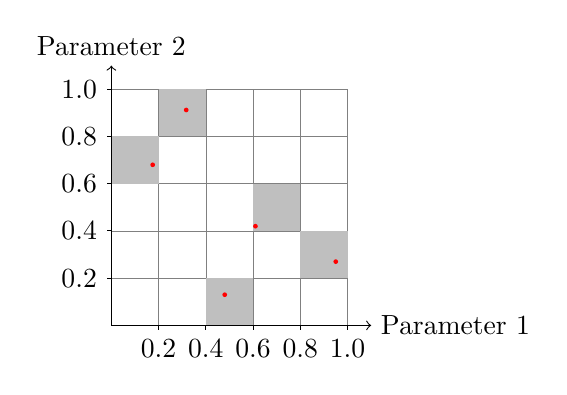
\begin{tikzpicture}[scale=3]

    % Define the grid
    \draw[step=0.2,gray,very thin] (0,0) grid (1,1);
    
    % Shade specific squares
    \fill[gray!50] (0.0,0.6) rectangle (0.2,0.8);
    \fill[gray!50] (0.2,0.8) rectangle (0.4,1.0);
    \fill[gray!50] (0.4,0.0) rectangle (0.6,0.2);
    \fill[gray!50] (0.6,0.4) rectangle (0.8,0.6);
    \fill[gray!50] (0.8,0.2) rectangle (1.0,0.4);
    
    % Draw red points
    \fill[red] (0.175,0.68) circle (0.01);  % Point in the first square
    \fill[red] (0.317,0.912) circle (0.01);  % Point in the second square
    \fill[red] (0.48,0.13) circle (0.01);  % Point in the third square
    \fill[red] (0.61,0.42) circle (0.01);  % Point in the fourth square
    \fill[red] (0.95,0.27) circle (0.01);  % Point in the fifth square
    
    % Draw the axes
    \draw[->] (0,0) -- (1.1,0) node[right] {Parameter 1};
    \draw[->] (0,0) -- (0,1.1) node[above] {Parameter 2};
    
    % Add ticks and labels
    \foreach \x in {0.2,0.4,0.6,0.8,1.0} {
      \draw (\x,0) -- (\x,-0.02) node[below] {\x};
      \draw (0,\x) -- (-0.02,\x) node[left] {\x};
    }
    
\end{tikzpicture}
    \caption{\acrshort{lhs} illustration}
    \label{fig:lhs}
\end{figure}

%// TODO: wait for results

%%%%%%%%%%%%%%%%%%%% BO Experiment %%%%%%%%%%%%%%%%%%%%%%%%%%
\subsection{\acrshort{bo} experiment}
\label{sec:bo_exp}

%// TODO: wait for results

Figure \ref{fig:exp12_res} depicts the performance of Bayesian Optimization (BO) over 50 iterations, measured in terms of the normalized Hellaswag accuracy (acc\_norm). This visualization highlights the evolution of the optimization process as it transitions from sampling to the exploitation, and ultimately converges towards high-performing solutions.


\begin{figure}[h!]
    \centering
    \begin{subfigure}[b]{.45\textwidth}
      \centering
      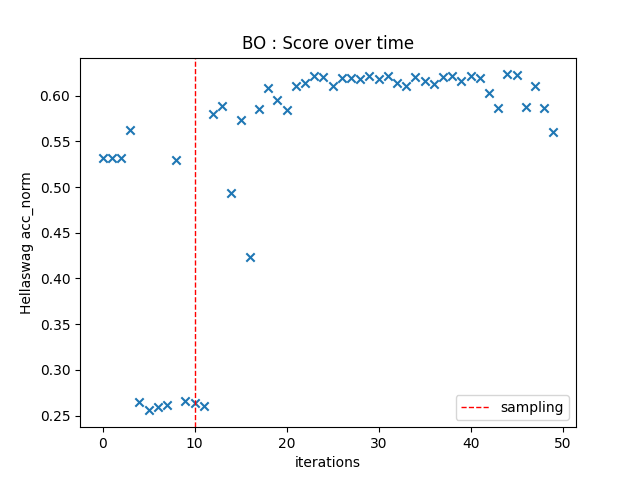
\includegraphics[height = 5cm]{assets/img/chap_4/experiments/plots/exp12_score_over_time.png}
      \caption{Score over time}
      \label{fig:exp12_score_time}
    \end{subfigure}%
    \begin{subfigure}[b]{.45\textwidth}
      \centering
      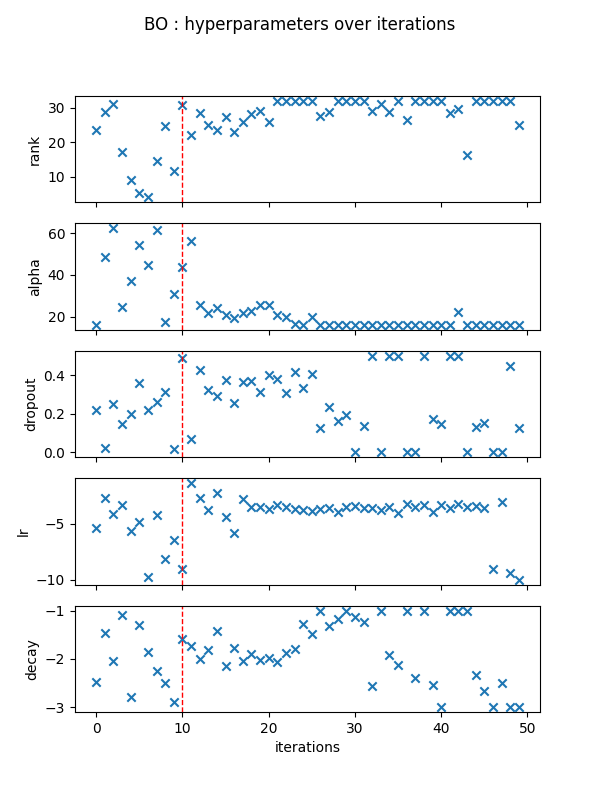
\includegraphics[height = 6cm]{assets/img/chap_4/experiments/plots/exp12_variables_over_time.png}
      \caption{Variable values over time}
      \label{fig:exp12_var_time}
    \end{subfigure}
    \caption{Experiment using \acrshort{bo} algorithm}
    \label{fig:exp12_res}
\end{figure}

During the sampling phase, as shown by figure \ref{fig:exp12_score_time} the best score achieved is at 56.27\% of normalized accuracy. This phase is interesting at is show us that there is a lot of area with good solution without exploitation. After this phase, there is around 15 iterations to converge to a stable phase, around 62\% of accuracy. After 40 iterations, the algorithm renew with a phase of exploration, to look if it's possible to achieve best results in others configuration, resulting in it's decrease in performance.

If we briefly look at figure \ref{fig:exp12_var_time}, it allow to look at well-chosen optimization range, or if it can be useful to enlarge it. For example, when looking at \acrshort{lora} rank, it's keeping it's value at the top of the range, implying that it would go up if possible. 

COMPARE WITH BOUNDS


To summarize, this experiment demonstrate the effectiveness of Bayesian Optimization in efficiently explore the search space. The optimization process strikes a balance between exploration and exploitation, achieving convergence within a limited number of iterations.


%%%%%%%%%%%%%%%%%%%% SOO Experiment %%%%%%%%%%%%%%%%%%%%%%%%%%
\subsection{\acrshort{soo} experiment}
\label{sec:soo_exp}
%// TODO: wait for results
Figure \ref{fig:exp11_res} depicts the performance of Simultaneous Optimistic Optimization (SOO) over 50 iterations, measured in terms of the normalized Hellaswag accuracy (acc\_norm). This visualization highlights the progression of the optimization process, showing limited improvement until later iterations, when a significant rise in performance is observed.

\begin{figure}[h!]
    \centering
    \begin{subfigure}[b]{.45\textwidth}
      \centering
      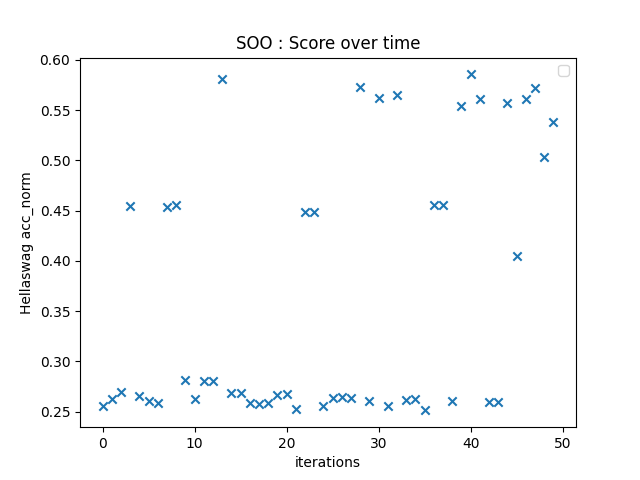
\includegraphics[height = 5cm]{assets/img/chap_4/experiments/plots/exp10_score_over_time.png}
      \caption{Score over time}
      \label{fig:exp11_score_time}
    \end{subfigure}%
    \begin{subfigure}[b]{.45\textwidth}
      \centering
      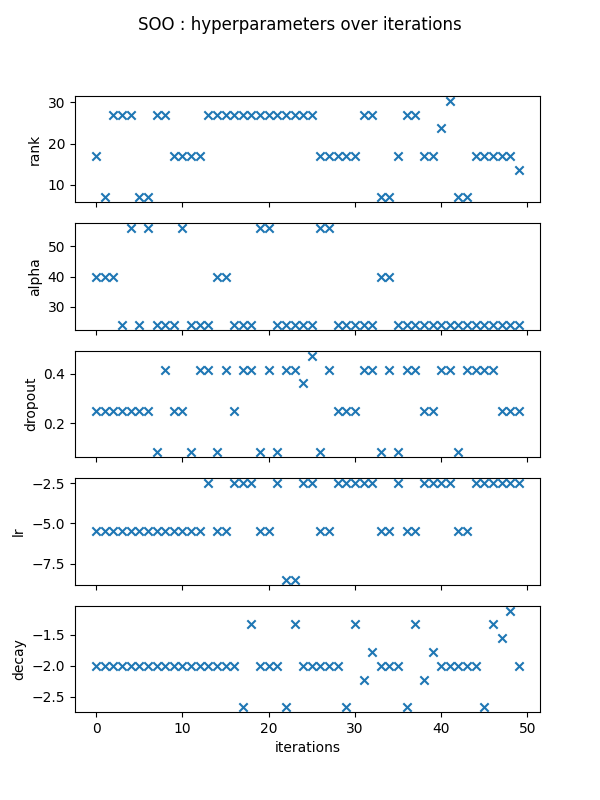
\includegraphics[height = 6cm]{assets/img/chap_4/experiments/plots/exp10_variables_over_time.png}
      \caption{Variables over time}
      \label{fig:exp11_var_time}
    \end{subfigure}
    \caption{Experiment using \acrshort{soo} algorithm}
    \label{fig:exp11_res}
\end{figure}

In the initial phase, spanning roughly the first 20 iterations, the accuracy remains relatively low and consistent, fluctuating around 0.25 to 0.3. This indicates that the SOO algorithm invests heavily in exploration during the early stage, sampling diverse regions of the parameter space but failing to identify high-performing regions.

Between iterations 20 and 40, a gradual improvement is observed as the algorithm transitions to exploitation. In this phase, SOO focuses on refining potential solutions, leading to a slight increase in accuracy, although the improvement remains modest compared to Bayesian Optimization.

In the final stage, after iteration 40, a significant rise in performance is observed, with accuracy values increasing sharply and converging around 0.6. This stabilization phase indicates that SOO successfully identifies high-quality parameter configurations, albeit at a slower pace compared to BO.

To summarize, Figure \ref{fig:exp11_res} demonstrates that SOO is capable of finding high-performing solutions but requires a longer exploration phase and slower convergence compared to Bayesian Optimization. Despite its delayed success, the eventual convergence highlights the potential of SOO for hyperparameter tuning tasks.

%%%%%%%%%%%%%%%%%%%% BaMSOO Experiment %%%%%%%%%%%%%%%%%%%%%%%%%%
\subsection{\acrshort{bamsoo} experiment}
\label{sec:bamsoo_exp}
%// TODO: wait for results
Figure \ref{fig:bamsoo_score_time} depicts the performance of Bamsoo over 50 iterations, measured in terms of the normalized Hellaswag accuracy (acc\_norm). This visualization highlights a hybrid approach that balances the rapid improvement seen in Bayesian Optimization (BO) and the thorough exploration typical of Simultaneous Optimistic Optimization (SOO).

\begin{figure}[h!] \centering 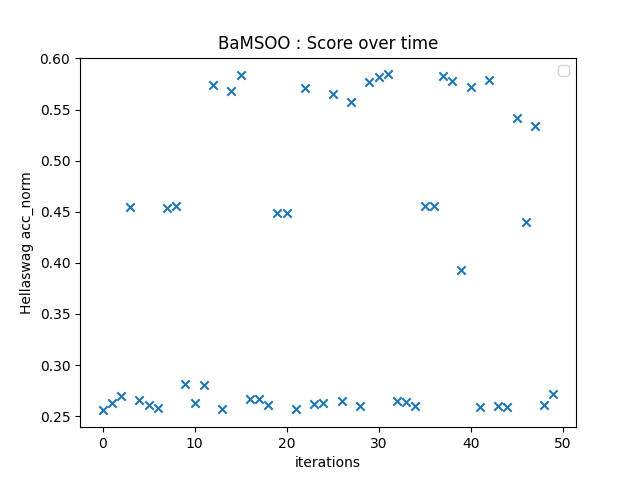
\includegraphics[width=0.4\linewidth]{assets/img/chap_4/experiments/plots/exp11_score_over_time.png} \caption{Score over time with \acrshort{bamsoo}} \label{fig:bamsoo_score_time} \end{figure}

In the initial phase, spanning the first 10 iterations, Bamsoo demonstrates an exploratory behavior similar to SOO. Accuracy values during this phase fluctuate around 0.25 to 0.3, indicating that the algorithm is sampling widely across the parameter space to gather foundational knowledge about the landscape.

Between iterations 10 and 30, the algorithm transitions to a phase of steady improvement, combining elements of exploration and exploitation. This phase is characterized by a gradual rise in accuracy, suggesting that Bamsoo refines its focus on promising regions of the parameter space while still allowing room for broader searches to avoid premature convergence.

In the final stage, after iteration 30, Bamsoo exhibits a stabilization phase with accuracy values consistently converging around 0.55 to 0.6. This indicates that the algorithm successfully identifies high-quality parameter configurations while maintaining the flexibility to avoid getting trapped in local optima.

To summarize, Figure \ref{fig:bamsoo_score_time} illustrates the hybrid nature of Bamsoo, which successfully balances exploration and exploitation across iterations. This behavior enables it to achieve competitive performance relative to BO and SOO, making Bamsoo a compelling alternative for optimization tasks requiring adaptability and robustness.

%%%%%%%%%%%%%%%%%%%%%%%%%% Analysis %%%%%%%%%%%%%%%%%%%%%%%%%%
\subsection{Comparison and analysis}
\label{sec:exp_analysis}
%// TODO - write this part
wait for results

%%%%%%%%%%%%%%%%%%%%%%%%%% Article Publication %%%%%%%%%%%%%%%%%%%%%%%%%%
\section{Article Publication}
\label{sec:article}

After few weeks of my internship, when we were able to define cleary a subject and estimate the possible contribution, with my supervisor we decided to aim to write an article from what I worked on. This aims push me to refine clearly what would be my contribution, since a published paper should aim for this. 

Under my supervisor guidance, what we aimed for was a conference article, for the International Conference on Optimization \& Learning (OLA2025). With this, a long paper will be published in \textit{Springer} indexed proceedings. At the time of writing and sending this report, the paper is under review, and the outcome is awaited. The current version can be found on github\footnote{\url{https://github.com/Kiwy3/ST30-report/blob/report/OLA.pdf}}

After a section on the contribution, I will adress in section \ref{sec:redaction} the redaction of the article, as it was also a crucial part of my internship.

%%%%%%%%%%%%%%%%%%%%%%%%%% Contribution %%%%%%%%%%%%%%%%%%%%%%%%%%
\subsection{The contribution}
\label{sec:contribution}
The first contribution of this work is direct and practical: the provision of usable \acrshort{hpo} algorithms and experiments specifically tailored for \acrshort{llm} \gls{fine_tuning}. The popularization of \acrshort{llm}s is a relatively recent development, and while these models are increasingly adopted by companies and end-users, the process of \gls{fine_tuning} remains somewhat inaccessible due to knowledge barriers and the lack of practical resources. By providing detailed experiments and insights into \acrshort{hpo} algorithms, this work aims to lower these barriers, enabling users to better understand and utilize \gls{fine_tuning} techniques. Furthermore, this contribution supports the selection of \glspl{hyperparameter}—a crucial step in achieving optimal performance without excessive trial and error.

The second contribution lies in addressing the challenge of optimizing expensive functions. The development and training of \acrshort{ann}s are computationally intensive processes, underscoring the importance of efficient optimization methods. This has driven significant interest in \acrshort{bo} algorithms, originally developed for scenarios such as mechanical and aeronautical engineering, where simulations can take hours to run. However, other domains with similarly expensive functions stand to benefit from advancements in this area. Through this work, a comparative analysis was conducted between two approaches for optimization in settings with limited evaluations, providing valuable insights for both researchers and practitioners.

Finally, this work contributes to the scalability of \acrshort{bo} algorithms. Given that this internship is part of an exascale computing project, the broader goal is to develop scalable and efficient algorithms capable of handling a wide variety of use cases. While the immediate focus has been on \acrshort{llm} \gls{fine_tuning}, the findings and methodologies have implications that extend to other computationally intensive tasks. By addressing scalability, this work lays the groundwork for future innovations in optimization methods that can leverage the full potential of high-performance computing infrastructure.


%%%%%%%%%%%%%%%%%%%%%%%%%% Redaction %%%%%%%%%%%%%%%%%%%%%%%%%%
\subsection{Redaction}
\label{sec:redaction}

%// TODO - write this part



%%%%%%%%%%%%%%%%%%%%%%%%%% Challenges %%%%%%%%%%%%%%%%%%%%%%%%%%
\section{Challenges}
\label{sec:challenge}
%// TODO - write this part

This section outlines the key challenges encountered during the internship and the strategies employed to address them. Undertaking a project situated at the intersection of multiple research domains presented unique difficulties, from defining and addressing a novel research problem to managing the technical complexities of implementation and resource constraints. Each of these challenges required a combination of critical thinking, adaptability, and collaboration to overcome. The following sections delve into these obstacles in detail, highlighting the learning process and the methods used to navigate the intricacies of both the theoretical and practical aspects of the work.



%%%%%%%%%%%%%%%%%%%%%%%%%% Complex field %%%%%%%%%%%%%%%%%%%%%%%%%%
\subsection{Adress a research problematic}
\label{sec:adress_research}
%// TODO - write this part
The first significant challenge I faced during the initial weeks of my internship was adapting to a completely new environment and working on a subject rooted in research—a domain I had not fully encountered before. While my academic courses had involved numerous projects of varying complexity and levels of research ambition, this internship marked the first time I was required to address a genuine research problem in its entirety. This shift introduced me to the complexities of the research process and the skills necessary to navigate it effectively.

One of the initial hurdles was managing the literature review. This involved handling numerous references, reading and analyzing complex academic articles, and extracting relevant information to identify a specific research problem. Estimating the right problematic to focus on proved particularly difficult at the outset, given the broad scope and technical depth of the subject. However, with the guidance of my supervisor, I was able to refine my understanding of the domain, define a clear and well-scoped research problem, and develop a structured approach to tackle it. This process laid the foundation for the rest of the project, ensuring that my efforts were focused and aligned with the goals of the internship.


%%%%%%%%%%%%%%%%%%%%%%%%%% Complex field %%%%%%%%%%%%%%%%%%%%%%%%%%
\subsection{Work in a complex research field}
\label{sec:complex_field}
%// TODO - write this part
The subject of my internship was as fascinating as it was complex, sitting at the intersection of several cutting-edge research fields. To approach this multidisciplinary challenge effectively, I began with a rapid yet thorough literature review of each relevant aspect. This step was essential to grasp the stakes of the subject and avoid wasting valuable time on unnecessary or redundant work. The fields I needed to familiarize myself with included \acrshort{llm}, encompassing \acrshort{ann}s and the specific nuances of \acrlong{peft}, as well as \acrlong{bo}, which required an understanding of probabilistic models and optimization rules. Additionally, I had to delve into \acrfull{hpc}, particularly the scalability of processes, which became increasingly relevant to my project’s objectives.

This endeavor was particularly challenging for me because my aim was to produce work comparable to that of well-established researchers or even research teams, despite having only a short internship period of six months to achieve it. Starting from scratch, I had to quickly acquire foundational knowledge and develop expertise in these domains. Balancing the demands of mastering multiple complex fields while striving to meet the high standards of professional research pushed me to adapt and learn at an accelerated pace. This experience, while demanding, was invaluable in helping me grow both academically and professionally.


%%%%%%%%%%%%%%%%%%%%%%%%%% Technical implementation %%%%%%%%%%%%%%%%%%%%%%%%%%
\subsection{Technical implementation}
\label{sec:tech_impl}
%// TODO - write this part


The first significant difficulty I encountered was related to the development process itself. I lacked a well-structured approach to code development, including strategies for writing clean, efficient, and modular code, as well as systematic methods for testing it. This absence of an established process initially slowed down my progress and required me to learn best practices as I advanced through the project.

Another major challenge was working with numerous libraries for implementing the black-box objective function. The codebase involved a complex network of libraries, classes, and functions, all deeply interconnected. It was initially overwhelming to understand how these components interacted and to adapt the existing code to fit my specific requirements. This was especially challenging because my use case—\acrlong{hpo}—was not a generic application of the libraries. As such, no pre-existing implementation was readily available to use \acrshort{hpo} as a black-box objective function, requiring significant effort to tailor the code.

Resource limitations also posed a considerable obstacle. At the beginning of the project, I had to rely on Grid'5000 as the primary computational resource. While g5k provided an essential platform for experimentation, its limitations in terms of scalability and availability required careful management of resources and computational tasks. Overcoming these challenges not only helped me refine my problem-solving skills but also provided valuable experience in navigating the practical constraints of real-world computational research.
